\section{Installation}

The repository at \url{https://github.com/datafl4sh/shimmer.git} includes shimmer++ library sources, the original matlab code on which shimmer++ is based (not a direct translation) and some documents related to the underlying physical model, along with the github issues that record the developments of shimmer++.  
\subsection{Getting your local copy of the repository}
As first step you should make sure that your system is up-to-date. For Debian-based operating systems: 
    \begin{verbatim}
        sudo apt update
    \end{verbatim}    
The next step is to install the dependencies which are SQLite, Eigen and the Boost Graph Library (BGL). SQLite is a file-based relational database used to store the gas networks, Eigen is concerned with the linear algebra and the BGL is a graph library used to represent the networks in-memory. The development environment for Shimmer++ is based on CMake and GCC or Clang. Shimmer++ is written in C++20, therefore a relatively recent compiler is needed.
For Debian-based operational system: 
\begin{verbatim}
    sudo apt install -y make cmake build-essential git ctest
    sudo apt install -y libsqlite3-dev lua5.4
    sudo apt install -y libeigen3-dev
    sudo apt install -y libboost-graph-dev libboost-dev
\end{verbatim}
   
You can now clone the Shimmer++ repository using
\begin{verbatim}        
    git clone https://github.com/datafl4sh/shimmer.git
\end{verbatim}
or, if you have write access
\begin{verbatim}
    git clone git@github.com:datafl4sh/shimmer.git
\end{verbatim}

\subsection{Building shimmer++}
To build shimmer++ use the standard ccmake/make steps knowing that the CMakeList.txt is in the shimmer++ directory.
\begin{verbatim}
    ccmake "path_to_shimmer++_directory"         
    make  
\end{verbatim}


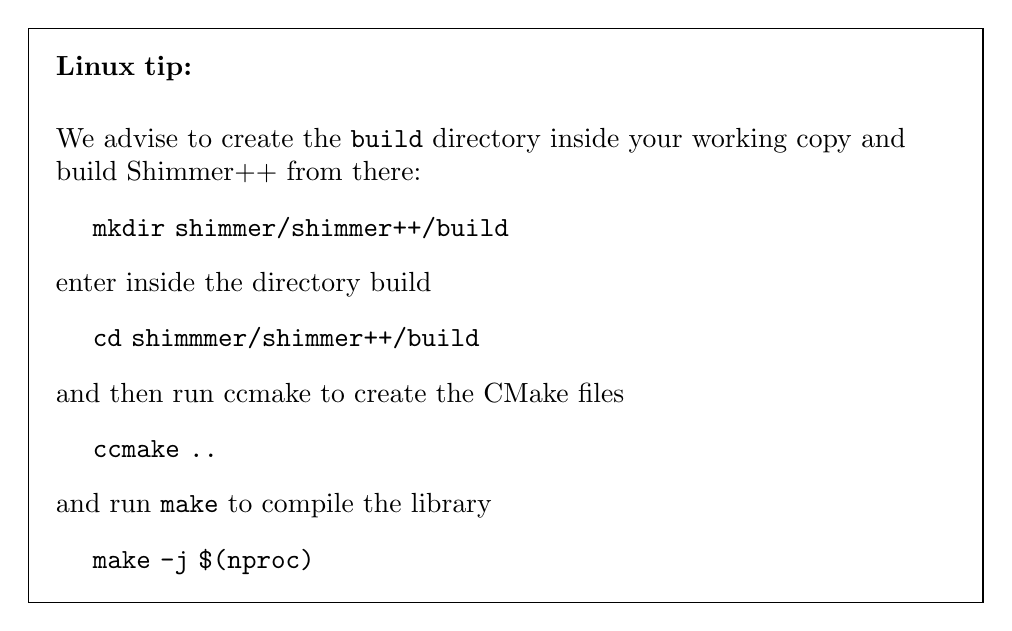
\begin{tikzpicture}
    \node [draw,text width=\linewidth-20pt, inner sep=10 pt]%
{
\textbf{Linux tip:}
\vspace{5mm} \\
We advise to create the \texttt{build} directory inside your working copy and build Shimmer++ from there:
\begin{verbatim}
    mkdir shimmer/shimmer++/build
\end{verbatim}
enter inside the directory build
\begin{verbatim}
    cd shimmmer/shimmer++/build
\end{verbatim}
and then run ccmake to create the CMake files
\begin{verbatim}
    ccmake ..
\end{verbatim}
and run \texttt{make} to compile the library
\begin{verbatim}
    make -j $(nproc)
\end{verbatim}
};
\end{tikzpicture}

\subsection{Running Shimmer++}
The database schema employed by the NDFs is provided in \texttt{shimmer/sqlite/shimmer.sql}. Assuming that you want to create a new NDF named \texttt{newndf.db} and that you have the NDF schema in the current folder, to initialize a new database:
\begin{verbatim}
    sqlite3 newndf.db < shimmer.sql
\end{verbatim}
The file `newndf.db` will subsequently need to be populated with all the relevant data.

\subsection{Shimmer++ organization}
The library is mainly organised with sources stored in the \texttt{shimmer/shimmer++/src} folder and unitary tests in the \texttt{shimmer/shimmer++/unit\_tests}. There is an additionally GERG folder which accounts for the interface of shimmer++ with the code regarding GERG computations.

%\begin{tikzpicture}
%    \node [draw,text width=\linewidth-20pt, inner sep=10 pt]
%{
%\textbf{Amateur tip (Linux):}
%\vspace{5mm} \\
%To add a new test, assuming it is written inside a file \texttt{my\_test.cpp}, you are asked to add the following lines into the \texttt{shimmer++/unit\_tests/CMakeLists.txt} in order to create the executable along with the other existent unitary tests.
%\begin{verbatim}
%        add_executable(my_test my_test.cpp ${SHIMMER_SOURCES_T})
%        target_link_libraries(my_test ${LINK_LIBS})
%        add_test(NAME my_test COMMAND my_test)
%\end{verbatim}
%};
%\end{tikzpicture}


